\documentclass[10pt]{article}
\usepackage[spanish]{babel}
\usepackage{graphicx}
\usepackage[usenames,dvipsnames]{xcolor}
\usepackage{color}

%codigos: \begin{abstract} \end{abstract} es resumen
%nueva pagina \newpage
%colores predefinidos : white, black, red, green, blue, cyan, magenta, yellow
%\textcolor{blue}{text}
%\color{blue!20!black!30!green}{Prueba} mezcla de colores, conviene manejar solo 2 colores, es mas manejable



\begin{document}
{\centering
{\Large{Escuela Superior Polit\'ecnica del Litoral\\Facultad de Ingenier\'ia en Electricidad y Computaci\'on\\}}
\vspace{0.6in}

\includegraphics[scale=0.5]{espol.png}\\
\vspace{0.8in}
{\LARGE \textbf{\color{blue}{Lenguajes de Programaci\'on\\\vspace{0.3in}Experiencias de cada lenguaje}}\\
\vspace{0.5in}

%------------------------------------------------------------------------------------------%
\newpage
\tableofcontents

%------------------------------------------------------------------------------------------%
\newpage
\begin{flushleft}
\section{Android}
\vspace{0.5in}
\begin{abstract}
\vspace{0.3in}
\large{Este es el primer trabajo de lenguajes de programaci\'on,para el cual las indicaciones fueron las de realizar un proyecto de aplicaci\'on m\'ovil, mas espec\'ifico en Android.\\
Hubieron algunas dificultades al principio, era algo nuevo para todos, a\'un no ten\'iamos clara la idea de lo que se har\'ia.\\
Entre algunas ideas, finalmente surgi\'o MY TWIN, algo que realmente nos pareci\'o novedoso y con alguna utilidad que se puede agregar a un dispositivo m\'ovil.\\
Se trabajo bastante con los recursos del tel\'efono y se hizo mucho \'enfasis en la proyecci\'on de tener un dispositivo con todo personalizado.}
\end{abstract}
\begin{center}
\vspace{0.5in}

\includegraphics[scale=0.7]{logo}
\end{center}
\end{flushleft}

%------------------------------------------------------------------------------------------%
\newpage
\begin{flushleft}
\subsection{Introducci\'on}

\normalsize
MY TWIN una aplicaci\'on dirigida a toda clase de usuario mediante la cual podr\'as crear tu propio avatar, el cual se convertir\'a en tu asesor personal de tareas.

Una aplicaci\'on la cual jugar\'a con los estados de \'animo de tu avatar, los cuales estar\'an definidos por las diferentes tareas que cumplir\'a. Esto es que la aplicaci\'on no solo ser\'a para entretenimiento tendr\'a una funcionalidad que buscar\'a ayudar al usuario de una manera diferente, entretenida y personalizada.\\

\subsection{Idea}
\subsubsection{Problem\'atica}
Muchas veces tenemos nuestro celular o cualquier dispositivo m\'ovil en al cual podemos programar para que nos notifique o nos recuerde algunas tareas, pero eso es todo lo que hace.\\
Buscabamos entonces una funcionalidad extra al tel\'efono y que a la vez sea agradable al ususario.\\
Todo comenz\'o con una lluvia de ideas, donde algunas fueron muy simples y de poca utilidad y otrass en cambio eran muy complicadas y sin prestar el mayor benefecio, as\'i finalmente surgi\'o My Twin, idea que nos agrad\'o por que era posible de llevar a la realidad y adem\'as mejorar\'ia la funcionalidad de nuestro dispositivo m\'ovil.\\
My Twin como un entretenido gemelo virtual.\\
\vspace{0.3in}
\begin{center}
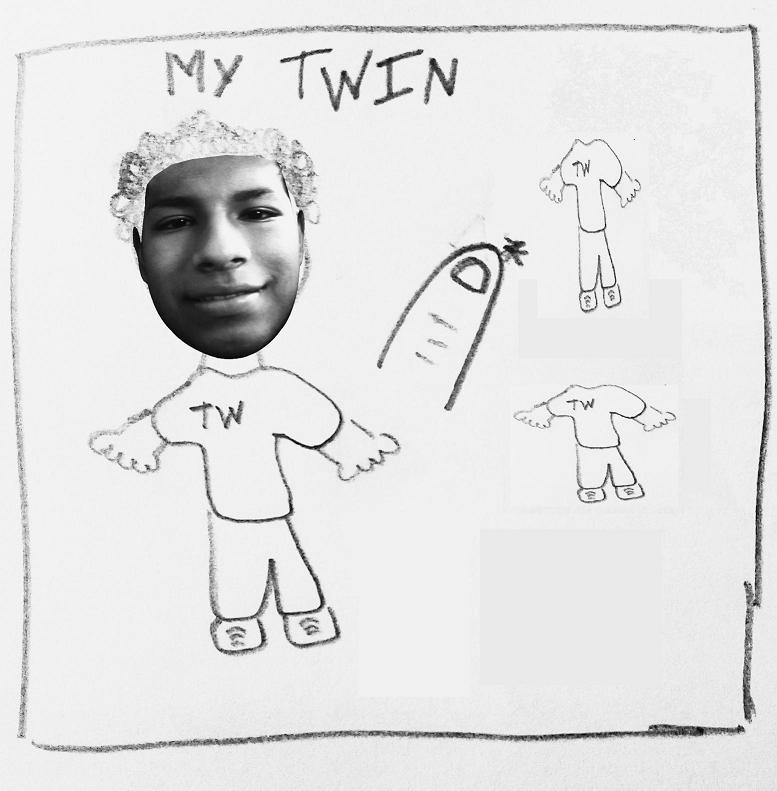
\includegraphics[scale=0.35]{bosquejoI1}
\end{center}

\end{flushleft}
}

%------------------------------------------------------------------------------------------%
\newpage
\begin{flushleft}
\subsubsection{Dise\~no}
El primer borrador fue trabajado en hojas con dibujos a mano, debido a que My Twin no era una sola pantalla est\'atica, sino que tiene algunas pantallas en la cual va cada una de las funciones.\\
Se dibujo algunos probables dise\~nos hasta llegar al que se tom\'o como modelo el siguiente.\\
\vspace{0.3in}
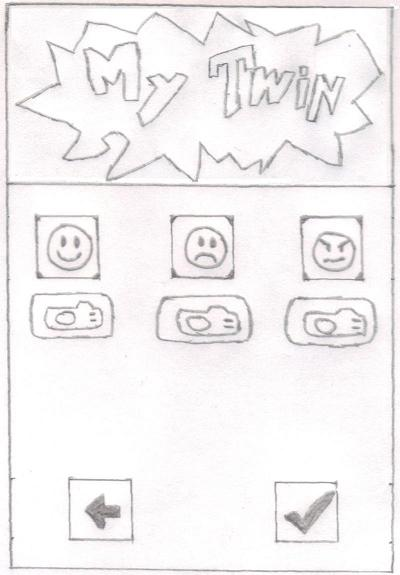
\includegraphics[scale=0.5]{Twin1}
\hspace{0.2in}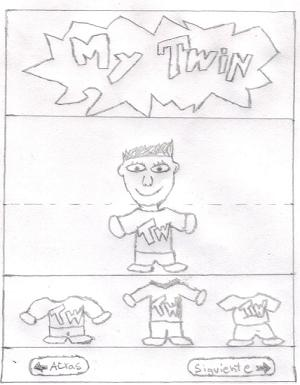
\includegraphics[scale=0.75]{Twin2}\vspace{0.2in}
\begin{center}
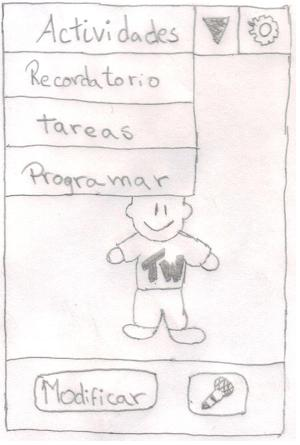
\includegraphics[scale=0.6]{Twin3}
\end{center}


\end{flushleft}


%------------------------------------------------------------------------------------------%
\newpage
\begin{flushleft}
\section{My Twin}
\subsection{Descripci\'on General}
\vspace{0.2in}
My Twin es una aplicaci\'on para dispositivo m\'ovil: \\\vspace{0.2in}\textbf{My Twin es divertido y original.\\
\vspace{0.1in}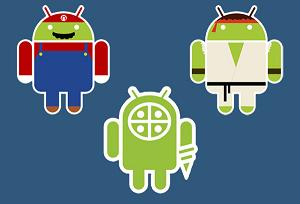
\includegraphics[scale=0.6]{3.jpg}\\
\begin{center}
\vspace{0.1in}My Twin es realista.\\
\vspace{0.1in}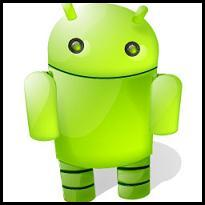
\includegraphics[scale=0.6]{droid.jpg}\\
\end{center}
\begin{flushright}
\vspace{0.1in}My Twin es amigable con el usuario.\\
\vspace{0.1in}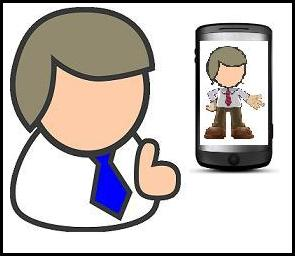
\includegraphics[scale=0.6]{amigableU.jpg}\\
\end{flushright}
}


\end{flushleft}

%------------------------------------------------------------------------------------------%
\newpage
\begin{flushleft}
\subsection{Funcionamiento(Manual de Usuario)}
\subsubsection{Pantalla Principal}

Pantalla Principal de My Twin, presionando en entrar, nos llevar\'a a la siguiente pantalla, si no tenemos aun creado el Twin, iremos a la pantalla de crear Twin, si ya lo tenemos, iremos directamente a la pantalla donde esta el menu y nuestro Twin.

\begin{center}
\vspace{0.1in}Pantalla Principal de inicio.\\
\vspace{0.1in}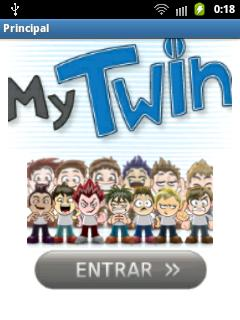
\includegraphics[scale=0.7]{PPrincipal}\\
\end{center}

\subsubsection{Creaci\'on de Twin}
Estas son las dos pantallas de creaci\'on del gemelo virtual, la primera es donde realizamos las fotos para la cara, d\'andole as\'i realismo; la segunda es para escoger un cuerpo, el cual le pone el lado original y divertido,donde todo es personalizable. \\
\begin{center}
\vspace{0.1in}
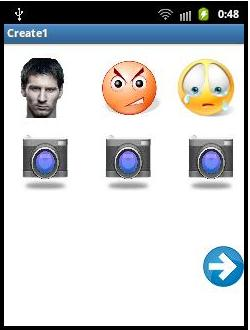
\includegraphics[scale=0.7]{create1.jpg}
\hspace{0.4in}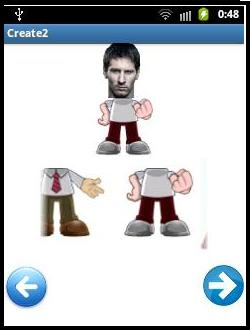
\includegraphics[scale=0.7]{create2.jpg}
\end{center}

\end{flushleft}



\end{document}